\subsection{Difference of Gaussian}
Difference of Gaussian, eller "DoG", er en
detektionsmetode introduceret  af David Lowe \cite{SIFT} og udgør feature detektoren i den samlede metode SIFT\footnote{Distinctive Image Features
from Scale-Invariant Keypoints}. "DoG" er en skala-invariant blob detektor, der definere et billede i skalarummet af det undersøgte billede foldet med et Gaussisk filter:
\begin{equation}
L(x,y,\sigma)= G(x,y,\sigma) \ast I(x,y)
\end{equation}
Metoden detektere punkter ved at lede efter ekstremaer i skala-rummet af "DoG" funktionen $ D(x,y,\sigma) $, hvilket kan udledes ved at tage forskellen imellem to nærliggende skalaer separeret af en en faktor $k=\sqrt{2}$, med en initial $\sigma$ værdi på $\sigma_0 = 1.6$, dvs. et givent skalabillede findes ved $\sigma_n=\sigma_0 \cdot k^n$:
\begin{equation}
\begin{split}
D(x,y,\sigma) &= (G(x,y,k\sigma)-(G(x,y,\sigma))\ast I(x,y) \\
           &= L(x,y,k \sigma)-L(x,y,\sigma)
\end{split}
\end{equation}
DoG er en blob detektor, da det er en approksimering til Laplacian of Gaussian eller "LoG" defineret som:
\begin{equation}
\begin{split}
LoG(x,y,\sigma) &= \sigma^2 \Delta^2L(x,y,\sigma) \\
                &= \sigma^2 (L_{xx}+L_{yy})
\end{split}
\end{equation}
Lowe relatere approksimeringen af DoG og LoG, ved varme-diffusion ligningen:
\begin{equation}
\dfrac{\partial L}{\partial \sigma} = \sigma \Delta^2L
\label{heat}
\end{equation}
Diffusions ligningen fra \eqref{heat}, kan approksimeres ved:
\begin{equation}
\begin{split}
\dfrac{\partial L}{\partial \sigma} &= \sigma \Delta^2L \\
&= \lim_{k \to 0} \dfrac{L(x,y,k\sigma)-L(x,y,\sigma)}{k\sigma-\sigma} \\
&\approx \dfrac{L(x,y,k\sigma)-L(x,y,\sigma)}{k\sigma-\sigma}
\end{split}
\label{difference}
\end{equation}
Yderligere kan \eqref{difference} udledes til,
\begin{equation}
\begin{split}
(k\sigma-\sigma)\sigma\Delta L &\approx L(x,y,k,\sigma)-L(x,y,\sigma) \\
(k-1)\sigma^2\Delta L &\approx L(x,y,k\sigma)-L(x,y,\sigma) \\
(k-1)\sigma^2LoG &\approx DoG
\end{split}
\end{equation}
Skalarummet deles op i $s$ oktaver, hvor der i overgangen imellem oktaver sker en fordobling af sigma værdien. For hver oktav indgår $s+3$ skala billeder, der hver iterativt foldes med et Gaussisk filter, med en sigma værdi ganget med en faktor $k$. Lowe anbefaler at bruge fire oktaver, hver med 7 skala billeder. I implementeringen er der brugt 4 oktaver, dog giver alle oktaver ikke brugbare interessepunkter og der anvendes derfor 5 skala billeder per. oktav, som er empirisk defineret til at give brugbare resultater. Når en oktav er fuldført, udvælges skalabillede nummer to, fra oktaven, dette billede nedsamples til halv størrelse og anvendes som første billede til næste oktav. De $s+3$ slørrede billeder, for hver oktav, subtrakteres med det første naboliggende skalabillede, som vist i figur \ref{fig:difference}(a) for at opnå "\textit{difference of gaussian}" billeder.
\begin{figure}[H]
    \centering
    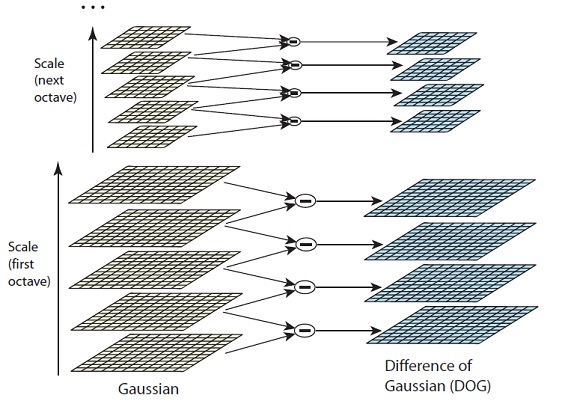
\includegraphics[width=0.65\textwidth]{fig/30.png}
     \vspace{-1em}
    \begin{center}    
       \caption{\textcolor{gray}{\footnotesize \textit{ }}}
    \label{fig:difference}
     \end{center}
     \vspace{-2.5em}
  \end{figure} \noindent
Dernæst udvælges lokale ekstremaer i "DoG" billederne, for hver pixel, ved at sammenligne et 3x3 pixel område i billedet med et 3$\times$3 pixel område i "DoG" billedet over, og under. Hvert pixel bliver derved sammenlignet med dens 27 naboer i de omkringliggende "DoG" billeder, hvor punktet bliver udvalgt til et ekstrema, hvis det er det mindste eller det største af disse, som illustreret i figur \ref{fig:difference}(b). Når lokale ekstremaer er udvalgt fravælges dårligt lokaliseret punkter f.eks. ekstremaer med lav kontrast, men også punkter, hvor ekstremaer ligger imellem pixels. Subpixels kan ikke direkte udvælges, men estimeres ved en Taylor udvidelse (af?) for at udvælge den korrekte subpixel position. Denne metode er introduceret af Brown og Lowe (citat 2002 måske) og kan opskrives som:
\begin{equation}
D(x)=D+\dfrac{\partial D^T}{\partial x}x\dfrac{1}{2}x^T\dfrac{\partial^2D}{\partial x^2}x
\end{equation}
Lokationen af ekstremaet $\hat{x}$ findes ved at tage den afledte af den ovenstående funktion ift. x og sætte den til 0:
\begin{equation}
\hat{x}= \dfrac{\partial^2 D^{-1}}{\partial x^2}\dfrac{\partial D}{\partial x}
\end{equation}
Er det lokale ekstrema lokaliseret med afstand $\hat{x}>0.5$ i en given dimension, vurderes det at punktet er lokaliseret tættere på et andet ekstrema, og punktet fjernes. Ustabile punkter med lav kontrast kan fjernes ved at sætte en grænseværdi for $ D(\hat{x}) $:
\begin{equation}
D(\hat{x})=D+\dfrac{1}{2}\dfrac{\partial D^T}{\partial x}\hat{x}
\end{equation}
Lowe foreslår at værdier af $D(\hat{x})$ under 0.03 fjernes. Metoden vil også have en positiv respons overfor kanter, derfor anvendes metoder lånt fra Harris og Stephens \cite{harris} til at fjerne disse. Hessian matricen opstilles som:
\begin{equation}
H =
\begin{bmatrix}
D_{xx} & D{xy} \\
D{xy} & D{yy}
\end{bmatrix}
\end{equation}
Hvor en grænseværdi for $r$ kan opstilles for at fjerne punkter lokaliseret på en kant:
\begin{equation}
\dfrac{tr(H)^2}{Det(H)}<\dfrac{(r+1)^2}{r}
\end{equation}
Punkter der tilfredsstiller denne grænseværdi udvælges som interessepunkter. 


\subsection*{Algoritme}
\begin{enumerate}
\item{Konstruer skalarummet for de forskellige oktaver, ved iterativt at folde skalabilledet med en stigende værdi af $\sigma$: $$ L(x,y,\sigma)= G(x,y,\sigma) \ast I(x,y) $$}
\item{Udregn "\textit{Difference of Gaussian}" billeder, ved at tage forskellen imellem skala billederne: $$ L(x,y,k \sigma)-L(x,y,\sigma)$$ }
\item{Lokaliser ekstremaer for hvert punkt i "\textit{Difference of Gaussian}" billeder, ved at sammenligne punktet med dens 27 naboer.}
\item{Afvis punkter der ikke er lokaliseret på ekstremaer, d.v.s. afvis punkter, der ikke opfylder følgende 
$$ \hat{x}<0.5 $$
Fjern punkter lokaliseret på ustabile ekstremaer ved at afvise punkter, der ikke opfylder:
$$ |D(\hat{x})|>0.03 $$}
\item{ Opstil Hessian matricen for at fjerne punkter lokaliseret på en kant: $$ \begin{bmatrix}
D_{xx} & D{xy} \\
D{xy} & D{yy}
\end{bmatrix} $$ 
og fjern punkter der ikke opfylder:
$$ \dfrac{tr(H)^2}{Det(H)}<\dfrac{(r+1)^2}{r}
$$
}
\end{enumerate}